% !TeX spellcheck = en_GB
\ifcsname SlidesDistr\endcsname%
\documentclass[handout,aspectratio=169]{beamer}
\else%
\documentclass[aspectratio=169]{beamer}
\fi%
\usepackage{fontspec}
\usepackage[T1]{fontenc}
\usepackage{amsmath}
\usepackage{amsfonts}
\usepackage{amssymb}
\usepackage{graphicx}
\usepackage{csquotes}
\usepackage{booktabs}
\usepackage{multicol}
\usepackage{enumerate}
\usepackage{microtype}
\usepackage[labelfont=bf,font={small}]{caption}
\usepackage{hyperref}
\usepackage{booktabs}
\usepackage{subcaption}
\usepackage{fancyhdr}
\usepackage{pdfpages}
\usepackage{siunitx}
\usepackage{tikz}
\usepackage{mdframed}

\defaultfontfeatures{Mapping=tex-text}
\newfontfamily\symbolfont{Symbola}
\newfontfamily\quotefont{GentiumPlus}

\usepackage[sorting=none]{biblatex}
\addbibresource{../bibliography.bib}

\author{Chris Eliasmith}


\renewcommand{\vec}[1]{{\mathbf{#1}}}
\newcommand{\mat}[1]{{\mathbf{#1}}}
\newcommand{\T}{\ensuremath{\mathsf{T}}}
\renewcommand{\epsilon}{\varepsilon}
\renewcommand{\phi}{\varphi}

% Tango color palette
\definecolor{butter1}{HTML}{FCE94F}
\definecolor{butter2}{HTML}{EDD400}
\definecolor{butter3}{HTML}{C4A000}
\definecolor{orange1}{HTML}{FCAF3E}
\definecolor{orange2}{HTML}{F57900}
\definecolor{orange3}{HTML}{CE5C00}
\definecolor{chocolate1}{HTML}{E9B96E}
\definecolor{chocolate2}{HTML}{C17D11}
\definecolor{chocolate3}{HTML}{8F5902}
\definecolor{chameleon1}{HTML}{8AE234}
\definecolor{chameleon2}{HTML}{73D216}
\definecolor{chameleon3}{HTML}{4E9A06}
\definecolor{skyblue1}{HTML}{729FCF}
\definecolor{skyblue2}{HTML}{3465A4}
\definecolor{skyblue3}{HTML}{204A87}
\definecolor{plum1}{HTML}{AD7FA8}
\definecolor{plum2}{HTML}{75507B}
\definecolor{plum3}{HTML}{5C3566}
\definecolor{scarletred1}{HTML}{EF2929}
\definecolor{scarletred2}{HTML}{CC0000}
\definecolor{scarletred3}{HTML}{A40000}
\definecolor{aluminium1}{HTML}{EEEEEC}
\definecolor{aluminium2}{HTML}{D3D7CF}
\definecolor{aluminium3}{HTML}{BABDB6}
\definecolor{aluminium4}{HTML}{888A85}
\definecolor{aluminium5}{HTML}{555753}
\definecolor{aluminium6}{HTML}{2E3436}

\definecolor{violet}{HTML}{AA305C}
\definecolor{uwyellow}{HTML}{FDD433}
\definecolor{background}{HTML}{F9F9F6}
\definecolor{text}{HTML}{000000}

\definecolor{uweng1}{HTML}{D1B2EE}
\definecolor{uweng2}{HTML}{BF33DE}
\definecolor{uweng3}{HTML}{8001B3}
\definecolor{uweng4}{HTML}{56048A}

\setbeamercolor{title}{fg=violet}
\setbeamercolor{frametitle}{fg=black}
\setbeamercolor{structure}{fg=aluminium5}
\setbeamercolor{normal text}{fg=text}

\setbeamertemplate{navigation symbols}{}
\setbeamertemplate{footline}[frame number]

\hypersetup{%
	colorlinks=false,% hyperlinks will be black
	urlbordercolor=aluminium4,% hyperlink borders will be red
	pdfborderstyle={/S/U/W 0.5}% border style will be underline of width 1pt
}

\makeatletter
\newcommand{\superimpose}[2]{%
	{\ooalign{{#1}\hidewidth\cr{#2}\hidewidth\cr}}}
\makeatother
\newcommand{\SolidCircle}[2]{\superimpose{\color{#1}\symbolfont ⬤}{\textbf{\color{white}#2}}\hspace{1em}}
\newcommand{\OPlus}{\SolidCircle{chameleon3}{\kern0.75pt+}}
\newcommand{\OMeh}{\SolidCircle{uwyellow}{~}}
\newcommand{\OMinus}{\SolidCircle{scarletred3}{\kern2.25pt--}}

\newcommand{\hl}[1]{\colorbox{uwyellow}{{\color{black}\textbf{#1}}}}

\newcommand{\ImageSources}[1]{%
	\begin{columns}%
		\column{1.1\textwidth}%
		\raggedright%
		\tiny\color{aluminium4}%
		\setlength\lineskip{1em}%
		\textbf{Image Sources.}	{#1}%
	\end{columns}}

\newcommand{\ColorRect}[3]{{\color{#1}\rule{#2}{#3}}}
\setbeamertemplate{headline}{\ColorRect{black}{\textwidth}{4pt}\newline\ColorRect{uweng1}{0.25\textwidth}{4pt}\ColorRect{uweng2}{0.25\textwidth}{4pt}\ColorRect{uweng3}{0.25\textwidth}{4pt}\ColorRect{uweng4}{0.25\textwidth}{4pt}}

\newcommand{\MakeTitle}{%
	\vspace{0.5cm}%
	{\textbf{\inserttitle}}\\[0.5cm]%
	\insertauthor\\[0.5cm]%
	\insertdate\\%
	\begin{itemize}
		\item Slide design: Andreas Stöckel
		\item Content: Terry Stewart, Andreas Stöckel, Chris Eliasmith
	\end{itemize}
 	\includegraphics[width=7cm]{../assets/uwlogo_eng.pdf}%
}

\newcommand{\handwritingframe}{%
	\begin{frame}
		\begin{columns}
			\column{\paperwidth}
			\includegraphics{../assets/handwriting_lines.pdf}
		\end{columns}
	\end{frame}	
}

\newcommand{\imageframe}[1]{%
	\setbeamertemplate{navigation symbols}{}%
	\begin{frame}[plain,noframenumbering]%
		\begin{tikzpicture}[remember picture,overlay]%
		\node[at=(current page.center)] {%
			\includegraphics[width=\paperwidth]{#1}%
		};%
		\end{tikzpicture}%
	\end{frame}%
}

\newcommand{\videoframe}[3][mp4]{%
	\begin{frame}[plain,noframenumbering]%
		\hypersetup{%
			pdfborderstyle={/S/U/W 0}% border style will be underline of width 1pt
		}%
		\begin{tikzpicture}[remember picture,overlay]%
		\node[at=(current page.center)] {%
			\includegraphics[width=\paperwidth]{{video/#2_#3}.jpg}%
		};%
		\node[at=(current page.center)] {%
			\ifcsname SlidesDistr\endcsname%
				\href{https://youtu.be/#3}{\includegraphics[width=2cm]{../assets/play_button.pdf}}%
			\else%
				\href{video/#2_#3.#1}{\includegraphics[width=2cm]{../assets/play_button.pdf}}%
			\fi%
		};%
		\end{tikzpicture}%
	\end{frame}%
}

\newcommand{\includevideo}[4][mp4]{%
	\begingroup%
	\hypersetup{%
		pdfborderstyle={/S/U/W 0}% border style will be underline of width 1pt
	}%
	\begin{tikzpicture}%
	\node (A) {%
		\includegraphics[width=#4]{{video/#2_#3}.jpg}%
	};%
	\node[at=(A.center)] {%
		\ifcsname SlidesDistr\endcsname%
			\href{https://youtu.be/#3}{\includegraphics[width=2cm]{../assets/play_button.pdf}}%
		\else%
			\href{video/#2_#3.#1}{\includegraphics[width=2cm]{../assets/play_button.pdf}}%
		\fi%
	};%
	\end{tikzpicture}%
	\endgroup%
}

\newcommand{\backupbegin}{
	\newcounter{finalframe}
	\setcounter{finalframe}{\value{framenumber}}
	\setbeamertemplate{footline}{}
}

\newcommand{\backupend}{
	\setcounter{framenumber}{\value{finalframe}}
}



\usepackage{ragged2e}

\date{Nov 6, 2023}
\title{SYDE 556/750 \\ Simulating Neurobiological Systems \\ Lecture 9: Analysing Representations}

\begin{document}
	
	\begin{frame}{}
		\vspace{0.5cm}
		\begin{columns}[c]
			\column{0.6\textwidth}
			\MakeTitle
			\column{0.4\textwidth}
			\includegraphics[width=\textwidth]{media/maurice_denis_homage_to_cezanne_1900_small.jpg}
		\end{columns}
	\end{frame}

	\begin{frame}{Decoding Polynomials}
		\centering
		\includegraphics[width=\textwidth]{media/poly_decodings.pdf} 
	\end{frame}

  \begin{frame}{Projection of the Neuron Space to PCA}
    \centering
    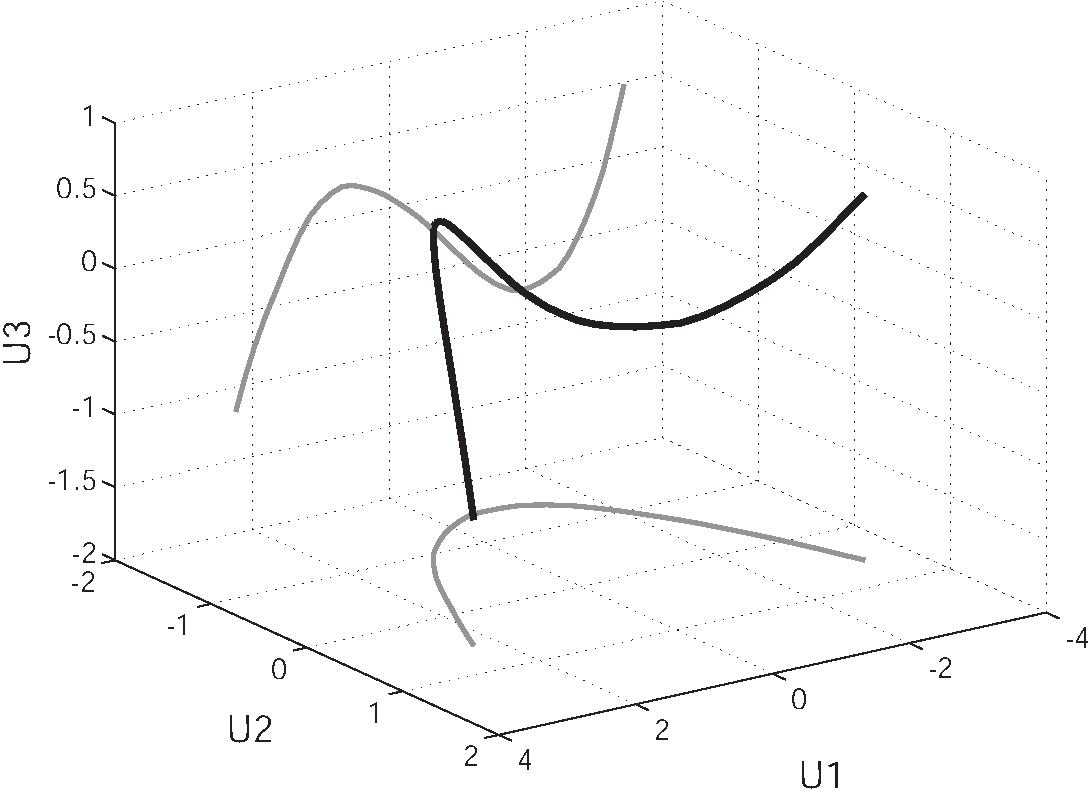
\includegraphics[scale=.4]{media/c5.chi.projections.pdf}
    
    A subspace of neuron activity being projected onto the first few principle component planes. Notice that the axis scales are different, capturing the size of the singular value.
  \end{frame}

	\begin{frame}{LIF Tuning Curve Principal Components}
		\centering
		\includegraphics[width=\textwidth]{media/tuning_curve_lif_pca.pdf}
		\begin{overlayarea}{\textwidth}{0.5cm}
			\centering
		\end{overlayarea}
	\end{frame}

	\begin{frame}{ReLU Tuning Curve Principal Components}
		\centering
		\includegraphics[width=\textwidth]{media/tuning_curve_relu_pca.pdf}
		\begin{overlayarea}{\textwidth}{0.5cm}
			\centering
			\only<2->{\hl{$\approx$ Legendre Basis}}
		\end{overlayarea}
	\end{frame}

	\begin{frame}{Reminder: Legendre Polynomials}
		\centering
		\includegraphics{media/legendre.pdf}
		\begin{align*}
			\phi_i(x)&= \frac{1}{2^i} \sum_{k=0}^n \binom{i}{k}^2 (x-1)^{i-k}(x+1)^k
		\end{align*}
		\begin{overlayarea}{\textwidth}{0.5cm}
			\centering
		\end{overlayarea}
	\end{frame}

	\begin{frame}{Modifying the Basis -- Same Maximum Rate (I)}
		\centering%
		\includegraphics<1>[width=\textwidth]{media/tuning_curve_relu_pca.pdf}%
		\includegraphics<2->[width=\textwidth]{media/tuning_curve_relu_pca_fix_max_rate.pdf}
		\begin{overlayarea}{\textwidth}{0.5cm}
			\centering
		\end{overlayarea}
	\end{frame}


	\begin{frame}{Modifying the Basis -- Equidistant $x$-Intercepts (II)}
		\centering%
		\includegraphics[width=\textwidth]{media/tuning_curve_relu_pca_fix_max_rate_intercepts_i.pdf}
		\begin{overlayarea}{\textwidth}{0.5cm}
			\centering
		\end{overlayarea}
	\end{frame}

	\begin{frame}{Modifying the Basis -- Limited $x$-Intercepts (III)}
		\centering%
		\includegraphics[width=\textwidth]{media/tuning_curve_relu_pca_fix_max_rate_intercepts_ii.pdf}
		\begin{overlayarea}{\textwidth}{0.5cm}
			\centering
		\end{overlayarea}
	\end{frame}

	\begin{frame}{Modifying the Basis -- Symmetric Tuning Curves (IV)}
		\centering%
		\includegraphics[width=\textwidth]{media/tuning_curve_relu_pca_symmetric.pdf}
		\begin{overlayarea}{\textwidth}{0.5cm}
			\centering
		\end{overlayarea}
	\end{frame}

	\begin{frame}{Gaussian Tuning Curve Principal Components}
		\centering
		\includegraphics[width=\textwidth]{media/tuning_curve_gaussian_pca.pdf}
		\begin{overlayarea}{\textwidth}{0.5cm}
			\centering
			\only<2->{\hl{$\approx$ Fourier Basis}}
		\end{overlayarea}
	\end{frame}

  \begin{frame}{Gaussian vs LIF Singular Values}
		\centering
		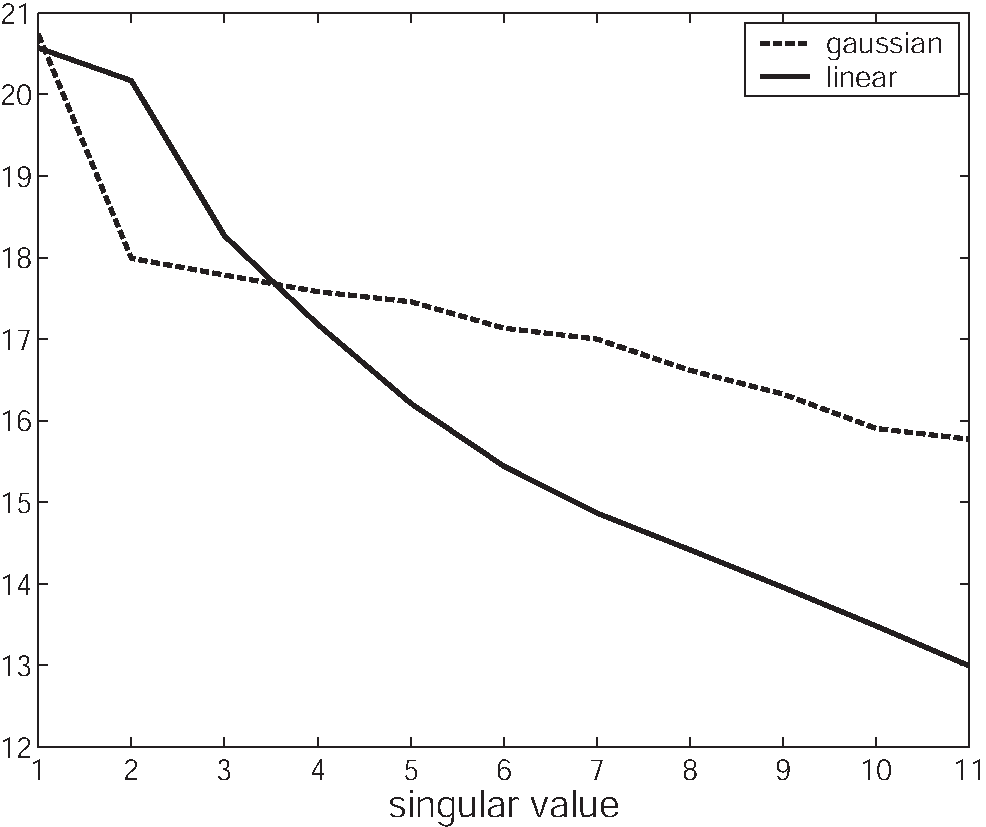
\includegraphics[scale=.5]{media/c5.line.gauss.sing.vals.pdf}
	\end{frame}

	\begin{frame}{PCA of 2D Tuning Curves}
		\centering
		\includegraphics[width=\textwidth]{media/2d_tuning_curves.pdf}
		\begin{overlayarea}{\textwidth}{0.5cm}
			\centering
			\only<2->{\vspace*{-0.5cm}\hl{Combination of 2D Polynomials}}
		\end{overlayarea}
	\end{frame}

  \begin{frame}{2D Singular Values}
		\centering
		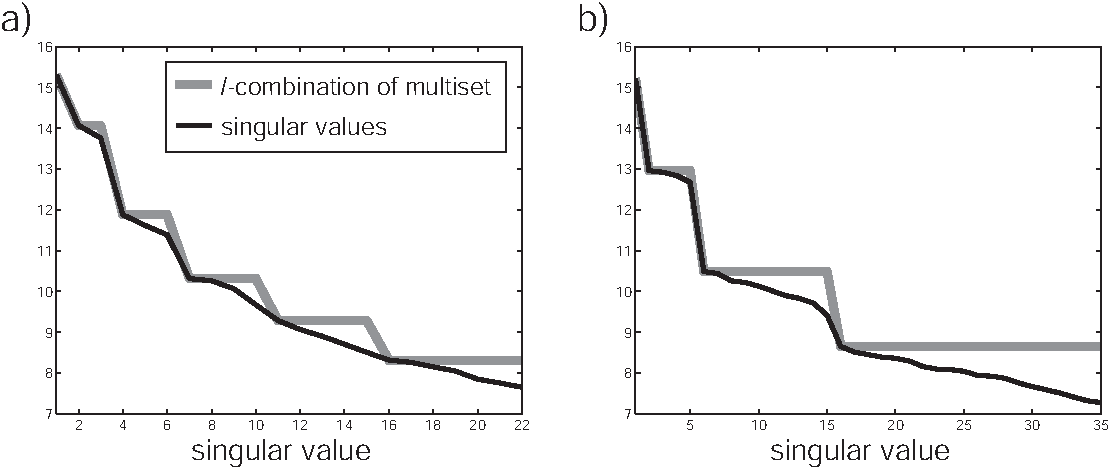
\includegraphics[scale=.5]{media/c5.multiset.2D.pdf}

    2D and 4D singular values compared to the prediction of the multiset (i.e., number of cross terms).
	\end{frame}

	\begin{frame}{Conclusions}
		\begin{itemize}
			\setlength{\itemsep}{0.5cm}
			\item Can use \hl{PCA} to find the basis functions underlying neural representations
			\item \hl{Singular values} inversely proportional to noise sensitivity
			\item \hl{Basis function shape} depends on\\[0.25cm]
			\begin{itemize}
				\setlength{\itemsep}{0.25cm}
				\item max firing rate distribution (a bit)
        \item $x$-intercept distribution
				\item neuron response curve $G[J]$
			\end{itemize}
			\item Finding optimal tuning curves for computing particular functions\\
			$\Rightarrow$ Full network optimization (must use gradient descent)
		\end{itemize}
	\end{frame}

	\backupbegin

	\begin{frame}[noframenumbering]{Image sources}
		\small
		\textbf{Title slide}\\Maurice Denis: Homage to Cézanne, 1900\\From \href{https://commons.wikimedia.org/wiki/File:Maurice_Denis_Homage_to_Cezanne_1900.jpg}{Wikimedia}.
	\end{frame}

	\backupend
	
\end{document}
